
% This LaTeX was auto-generated from MATLAB code.
% To make changes, update the MATLAB code and republish this document.

\documentclass{article}
\usepackage{graphicx}
\usepackage{color}

\sloppy
\definecolor{lightgray}{gray}{0.5}
\setlength{\parindent}{0pt}

\begin{document}

    
    
\subsection*{Contents}

\begin{itemize}
\setlength{\itemsep}{-1ex}
   \item Density Plot
\end{itemize}
\begin{verbatim}
G = sparse(nx*ny);
F = zeros(nx*ny,1);

for i = 1:nx
    for j = 1:ny

        n = j + (i-1)*ny; % node mapping

        if i == 1 % left side = V_0

            G(n,n) = 1;
            F(n) = V_0;

        elseif i == nx % right side = 0V

            G(n,n) = 1;
            F(n) = 0;

        elseif j == ny % top side = insulated

            % only three resistors:
            % n(x-1,y), n(x+1,y), n(x,y-1)

            nxm = j + (i-2)*ny;
            nxp = j + i*ny;
            nym = (j-1) + (i-1)*ny;

            G(n,n) = -3;
            G(n,nxm) = 1;
            G(n,nxp) = 1;
            G(n,nym) = 1;

        elseif j == 1 % bottom side = insulated

            % only three resistors:
            % n(x-1,y), n(x+1,y), n(x,y+1)

            nxm = j + (i-2)*ny;
            nxp = j + i*ny;
            nyp = (j+1) + (i-1)*ny;

            G(n,n) = -3;
            G(n,nxm) = 1;
            G(n,nxp) = 1;
            G(n,nyp) = 1;

        else % middle node

            nxm = j + (i-2)*ny;
            nxp = j + i*ny;
            nym = (j-1) + (i-1)*ny;
            nyp = (j+1) + (i-1)*ny;

            % middle nodes in G, based on the sum of four neighbour cells
            G(n,n) = -4;
            G(n,nxm) = 1;
            G(n,nxp) = 1;
            G(n,nym) = 1;
            G(n,nyp) = 1;

        end

    end
end

V = G\F;

% Map voltages back into a matrix

Vmap = zeros(nx,ny); % initialize matrix
n = 0; % clear/reset node index n

for i = 1:nx
    for j = 1:ny
        n = j + (i-1)*ny;
        Vmap(i,j) = V(n);
    end
end

Ex = [];
Ey = [];

for i = 1:nx
    for j = 1:ny

        % Calculate Ex
        if i == 1
            Ex(i,j) = Vmap(i+1,j) - Vmap(i,j);
        elseif i == nx
            Ex(i,j) = Vmap(i,j) - Vmap(i-1,j);
        else
            Ex(i,j) = (Vmap(i+1,j) - Vmap(i-1,j)) / 2.0;
        end

        % Calculate Ey
        if j == 1
            Ey(i,j) = Vmap(i,j+1) - Vmap(i,j);
        elseif j == ny
            Ey(i,j) = Vmap(i,j) - Vmap(i,j-1);
        else
            Ey(i,j) = (Vmap(i,j+1) - Vmap(i,j-1)) / 2.0;
        end

    end
end

Ex = -Ex;
Ey = -Ey;
Exy = sqrt(Ex.^2 + Ey.^2);

figure(1)
surf(Vmap) % plot surface
title('Electrostatic charge of Region')
view(135,45) % adjust camera angle for better view

figure(2)
subplot(2,1,1); surf(Exy);
axis([0 nx 0 ny])
title('Electric Field')
view(2) % view 2D plot
subplot(2,1,2); quiver(Ex,Ey);
axis([0 nx 0 ny])
\end{verbatim}

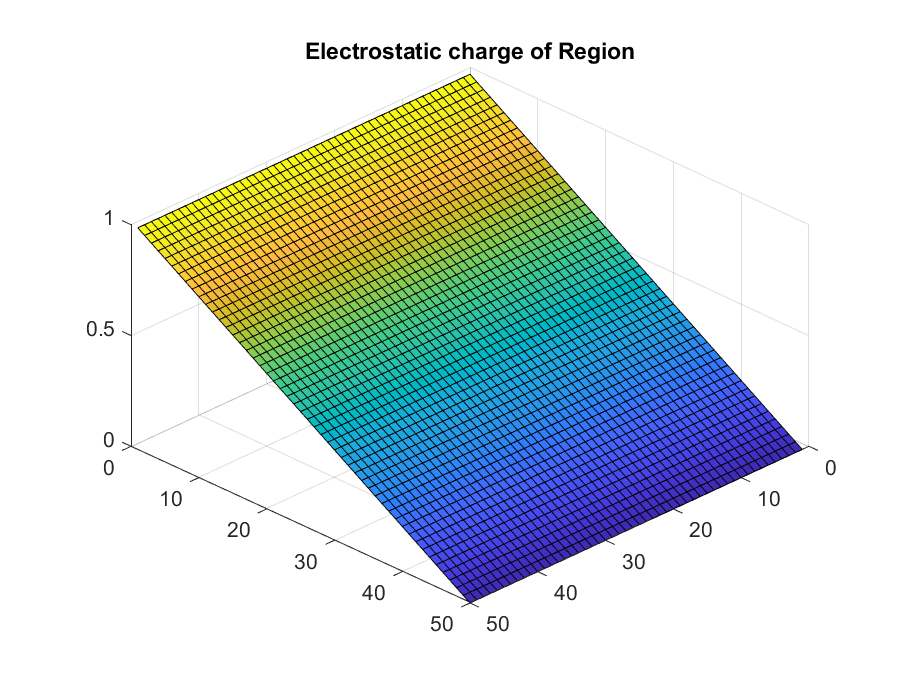
\includegraphics [width=4in]{assign3part1_01.eps}

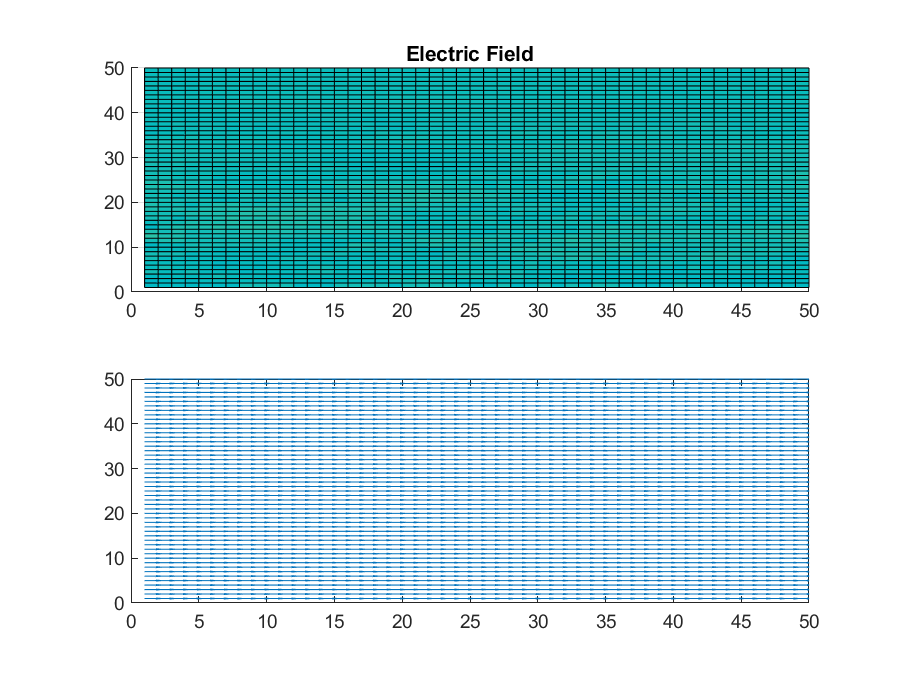
\includegraphics [width=4in]{assign3part1_02.eps}
\begin{par}
The above plot displays the electric field across the area. When we take the average E-field in the system, we see that it is a constant 0.0204 V/m.
\end{par} \vspace{1em}
\begin{verbatim}
avgEField = mean(Exy,'all');
\end{verbatim}
\begin{par}
Calculate the x and y forces induced by the electric field \$ E = \ensuremath{\backslash}frac\{F\}\{q\} \$, we can rewrite this to: \$ F = qE \$. Where q is the elementary charge. We take the mean to use as a constant across the area.
\end{par} \vspace{1em}
\begin{verbatim}
Fx = q*Ex*10^9;
Fy = q*Ey*10^9;
Fxy = q*Exy*10^9;
\end{verbatim}
\begin{par}
The force on the electrons is: \$ F = 2.3121e-11 \$. This checks out as we had just saw that the E-field in the region is constant everywhere.
\end{par} \vspace{1em}
\begin{verbatim}
avgFx = mean(Fx, 'all');
avgFy = mean(Fy, 'all');
\end{verbatim}
\begin{par}
With the force of the electric field determined, we can start simulating the movement of electrons in the semiconductor crystal. Previously, we looked at electrons with 0 acceleration. Now, we will use Newton's law to determine the new velocity from the previous velocity.
\end{par} \vspace{1em}
\begin{verbatim}
xPos = regL*rand(1,numElec);
yPos = regW*rand(1,numElec);

xVel = sqrt(3*kb * T/m_n)*randn(1,numElec);
yVel = sqrt(3*kb * T/m_n)*randn(1,numElec);
\end{verbatim}
\begin{par}
From Newton's law, we find that the acceleration is: \$ a = 1.3805e+18 \$.
\end{par} \vspace{1em}
\begin{verbatim}
accel = (mean(Fxy,'all')/m_n); % acceleration

Pscat = 1 - exp(-dt/t_mn); % Probability of scattering
\end{verbatim}
\begin{par}
Current is the flow of charge through an area. We often use current density, where \$ I = J\ensuremath{\tilde{\;}}\ensuremath{\backslash}times\ensuremath{\tilde{\;}}Area $. Thus, if we know the velocity of electrons, we should know the current density.\\ Current can also be described as the differential charge over differential time: $$ J\_x = \ensuremath{\backslash}frac\{\ensuremath{\backslash}delta q\}\{A \ensuremath{\backslash}delta t\} $$ We can rewrite the differential charge as: $$ e n A v\_\{dx\} \ensuremath{\backslash}delta t $$ Thus, we write our drift current density equation as: $$ J\_x = env\_\{dx\} \$\$ Where \$ e\ensuremath{\tilde{\;}}= \$ elementary charge, \$ n\ensuremath{\tilde{\;}}= \$ carrier concentration, and \$ v\_\{dx\}\ensuremath{\tilde{\;}}= \$ x-direction velocity. To calculate current, we will assume a carrier concentration of \$ 10\^{}\{15\}cm\^{}\{-2\} \$
\end{par} \vspace{1em}
\begin{verbatim}
carrierCon = 10e15; %cm^-2

index = 1;

for t = 1:numTimeStep

    figure(3)
    for n = 1:numDispElec
        plot(xPos(n), yPos(n),'.','color',Cols(n,:))
    end
    title('Electrons as Carriers in N-type Si crystal (with Collision)')
    axis([0 regL 0 regW])
    hold on

    carriers = (carrierCon*100^2)*(regL*regW/10^(-9*2));

    xCurrDens = q*carriers*xVel*dt;
    yCurrDens = q*carriers*yVel*dt;
    Jx = mean(xCurrDens); % current density
    Jy = mean(yCurrDens);
    Jxy(index) = sqrt(Jx^2 + Jy^2);

    randNum = rand(1, numElec); % generate a random number for each electron
    scatter = randNum < Pscat; % determine if electron scatters
    xVel(scatter) = sqrt(3*kb * T/m_n)*randn;
    yVel(scatter) = sqrt(3*kb * T/m_n)*randn;

    xVel = accel*dt + xVel;
    yVel = accel*dt + yVel;

    newXPos = xPos + xVel*dt;
    newYPos = yPos + yVel*dt;

    crossRight = newXPos >= regL;
    crossLeft = newXPos <= 0;
    xPos = xPos + xVel*dt;
    xPos(crossRight) = 0;
    xPos(crossLeft) = regL;

    crossTop = newYPos > regW;
    crossBottom = newYPos < 0;
    yVel(crossTop) = -yVel(crossTop);
    yVel(crossBottom) = -yVel(crossBottom);
    yPos = yPos + yVel*dt;

    index = index + 1;

%     pause(0.01);

end

time = linspace(0,dt*numTimeStep,numTimeStep);

figure(4)
plot(time,Jxy)
title('Current Density Over Time')
xlabel('Time')
ylabel('Current Density')
\end{verbatim}

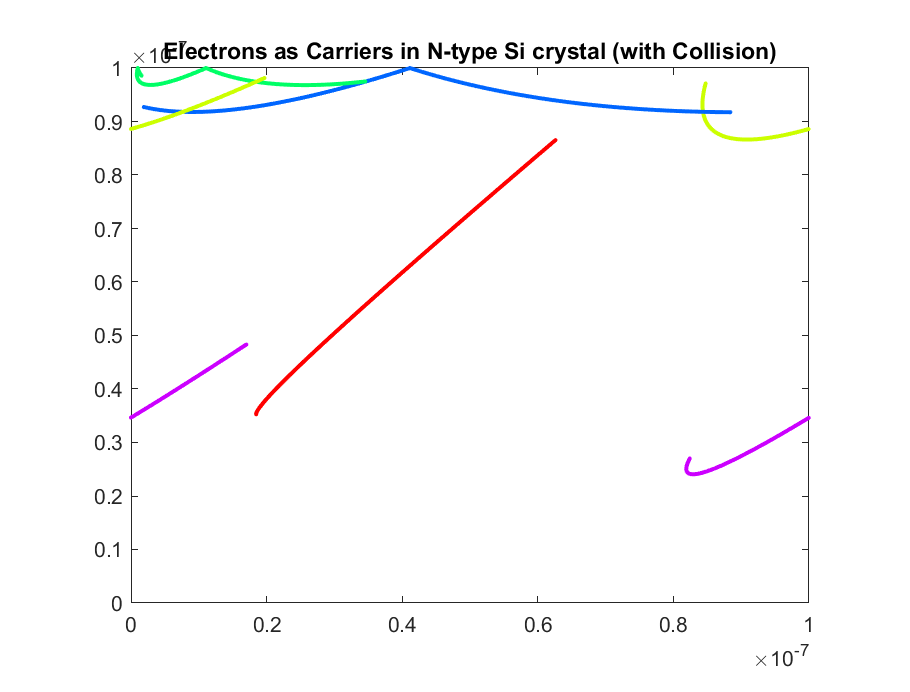
\includegraphics [width=4in]{assign3part1_03.eps}

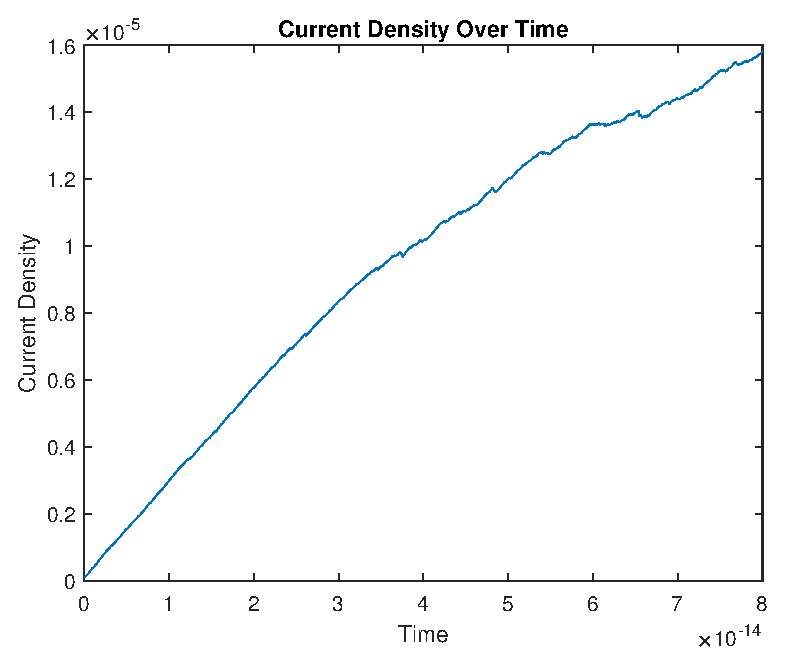
\includegraphics [width=4in]{assign3part1_04.eps}
\begin{par}
As the simulation progresses, we see the electrons begin to tend towards the right side of the region. This makes intuitive sense as their is an applied potential on the region where x = 0 is at a higher potential than x = 100nm. Thus, we see the current density steadily increase over time and then round off around 0.015mA. There is a little noise in the signal due to the scattering of the electrons as well, however the effect is quite minimal in comparison to the applied voltage.
\end{par} \vspace{1em}


\subsection*{Density Plot}

\begin{par}
After the completion of the simulation, we can take the final positions of the electrons and create a density plot. To do this, we divide the region into a meshgrid, loop through each differential area and count the number of electrons in that area creating a matrix of the number of electrons located in each segment of the region. This matrix can be plotted as a surface to help us visualize the electron density of the area.
\end{par} \vspace{1em}
\begin{par}
xPos and yPos now hold the final x and y positions of the electrons respectively. nx and ny (declared in main) are the number of segments the x and y directions will be divided into - thus the region will be divided into nx*ny smaller areas. We can divide the electrons x and y positions by the length and width and multiply by nx and ny respectively to obtain the index in which each electron resides in (these will have to be rounded up such that we are left with only whole integer values)
\end{par} \vspace{1em}
\begin{verbatim}
xi = ceil(xPos/regL*nx); % x index
yi = ceil(yPos/regW*ny); % y index

% loop through each smaller area and count the number of electrons present
for i = 1:nx
    for j = 1:ny

        match = (xi==i) & (yi==j); % search for all electrons at the current i,j index

        % match will have a 1 for every electron located at current index,
        % taking the sum gives the total number of electrons located at
        % this cell in the meshgrid
        sum_e = sum(match);

        densityPlot(i,j) = sum_e; % save this sum into a matrix to be mapped out

    end
end

densityPlot = densityPlot';

figure(5)
surf(densityPlot','EdgeColor','interp', 'FaceColor', 'interp')
view(2)
title('Density Plot')

% Plot temperature map
% use final velocities of electrons

E_k = m_n .* (sqrt(xVel.^2 + yVel.^2).^2) ./ 2;
Temp = (2.*E_k)./(3*kb);
avgTemp = mean(Temp);

tempMap = densityPlot.*avgTemp;
tempMap = tempMap';

figure(6)
s = pcolor(tempMap)
s.FaceColor = 'interp';
title('Temperature Plot')
\end{verbatim}

        \color{lightgray} \begin{verbatim}
s = 

  Surface with properties:

       EdgeColor: [0 0 0]
       LineStyle: '-'
       FaceColor: 'flat'
    FaceLighting: 'flat'
       FaceAlpha: 1
           XData: [1×50 double]
           YData: [50×1 double]
           ZData: [50×50 double]
           CData: [50×50 double]

  Use GET to show all properties

\end{verbatim} \color{black}
    
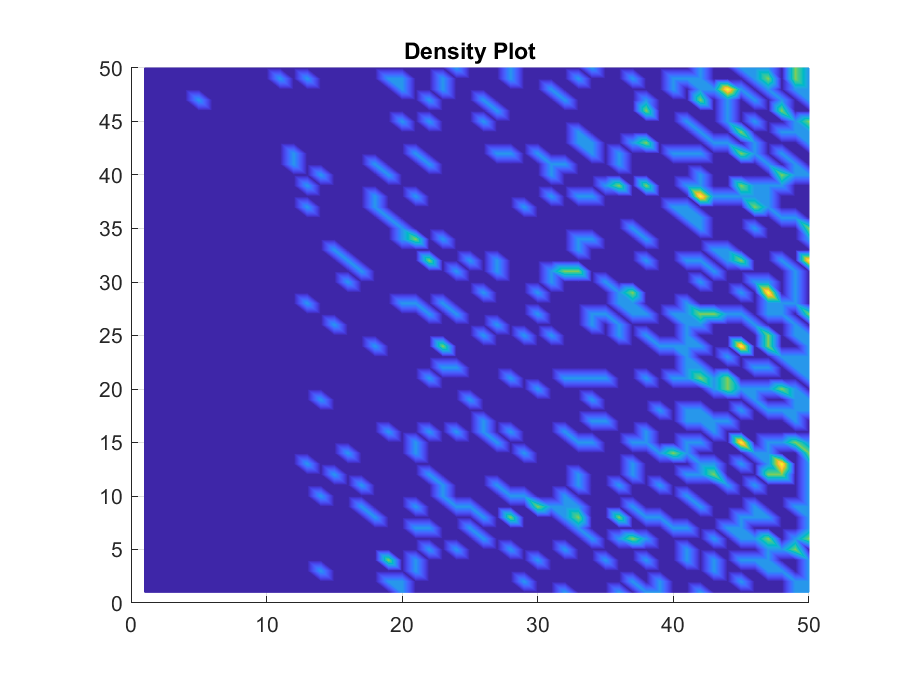
\includegraphics [width=4in]{assign3part1_05.eps}

\includegraphics [width=4in]{assign3part1_06.eps}



\end{document}

